% questions.tex —— 2015 年·全国Ⅰ卷·理科 · 题目内容片段（无答案）
% 由 tools/generate_projects.py 依来源总账自 2015/2015_数学真题_全国1理_试题.md 生成，勿手改（改源 MD 后重跑）


\begin{gktip}
依据固定原卷照录。图稿是源图的矢量描绘；原卷未标注各题分值、满分或时长，不补写。
\end{gktip}

\gkpart{一、选择题}

\begin{question}
\gkti{1}设复数 $z$ 满足 $\dfrac{1+z}{1-z}=\mathrm{i}$，则 $|z|=$（　）

(A) $1$　 (B) $\sqrt2$　 (C) $\sqrt3$　 (D) $2$

\end{question}
\begin{question}
\gkti{2}$\sin20^\circ\cos10^\circ-\cos160^\circ\sin10^\circ=$（　）

(A) $-\dfrac{\sqrt3}{2}$　 (B) $\dfrac{\sqrt3}{2}$　 (C) $-\dfrac12$　 (D) $\dfrac12$

\end{question}
\begin{question}
\gkti{3}设命题 $p:\exists n\in\mathbb N,\ n^2>2^n$，则 $\neg p$ 为（　）

(A) $\forall n\in\mathbb N,\ n^2>2^n$　 (B) $\exists n\in\mathbb N,\ n^2\leqslant2^n$

(C) $\forall n\in\mathbb N,\ n^2\leqslant2^n$　 (D) $\exists n\in\mathbb N,\ n^2=2^n$

\end{question}
\begin{question}
\gkti{4}投篮测试中，每人投 $3$ 次，至少投中 $2$ 次才能通过测试．已知某同学每次投篮投中的概率为 $0.6$，且各次投篮是否投中相互独立，则该同学通过测试的概率为（　）

(A) $0.648$　 (B) $0.432$　 (C) $0.36$　 (D) $0.312$

\end{question}
\begin{question}
\gkti{5}已知 $M(x_0,y_0)$ 是双曲线 $C:\dfrac{x^2}{2}-y^2=1$ 上的一点，$F_1,F_2$ 是 $C$ 的两个焦点．若 $\overrightarrow{MF_1}\cdot\overrightarrow{MF_2}<0$，则 $y_0$ 的取值范围是（　）

(A) $\left(-\dfrac{\sqrt3}{3},\dfrac{\sqrt3}{3}\right)$　 (B) $\left(-\dfrac{\sqrt3}{6},\dfrac{\sqrt3}{6}\right)$

(C) $\left(-\dfrac{2\sqrt2}{3},\dfrac{2\sqrt2}{3}\right)$　 (D) $\left(-\dfrac{2\sqrt3}{3},\dfrac{2\sqrt3}{3}\right)$

\Needspace{0.4\textheight}
\end{question}
\begin{question}
\gkti{6}《九章算术》是我国古代内容极为丰富的数学名著，书中有如下问题：“今有委米依垣内角，下周八尺，高五尺．问：积及为米几何？”其意思为：“在屋内墙角处堆放米（如图，米堆为一个圆锥的四分之一），米堆底部的弧长为 $8$ 尺，米堆的高为 $5$ 尺，问米堆的体积和堆放的米各为多少？”已知 $1$ 斛米的体积约为 $1.62$ 立方尺，圆周率约为 $3$，估算出堆放的米约有（　）
\nopagebreak[4]
\begin{center}% source-figure:q06-rice, fixed science PDF p.1 / printed 961.
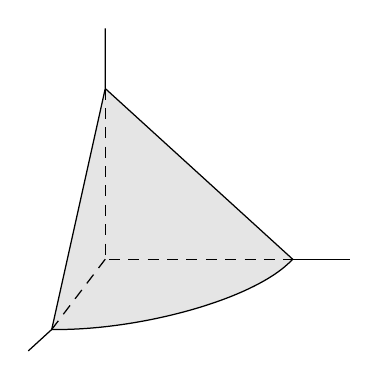
\begin{tikzpicture}[line width=.45pt,scale=.85]
  \fill[gray!20] (0,2.8) -- (-.8,-.8)
    .. controls (.5,-.82) and (2.25,-.35) .. (2.8,.25) -- cycle;
  \draw (0,3.7) -- (0,2.8) -- (-.8,-.8)
    .. controls (.5,-.82) and (2.25,-.35) .. (2.8,.25) -- (0,2.8);
  \draw (-1.15,-1.12) -- (-.8,-.8);
  \draw (2.8,.25) -- (3.65,.25);
  \draw[dash pattern=on 4pt off 3pt] (0,2.8) -- (0,.25) -- (2.8,.25);
  \draw[dash pattern=on 4pt off 3pt] (0,.25) -- (-.8,-.8);
\end{tikzpicture}
\end{center}
\nopagebreak[4]
(A) $14$ 斛　 (B) $22$ 斛　 (C) $36$ 斛　 (D) $66$ 斛

\end{question}
\begin{question}
\gkti{7}设 $D$ 为 $\triangle ABC$ 所在平面内一点，$\overrightarrow{BC}=3\overrightarrow{CD}$，则（　）

(A) $\overrightarrow{AD}=-\dfrac13\overrightarrow{AB}+\dfrac43\overrightarrow{AC}$　 (B) $\overrightarrow{AD}=\dfrac13\overrightarrow{AB}-\dfrac43\overrightarrow{AC}$

(C) $\overrightarrow{AD}=\dfrac43\overrightarrow{AB}+\dfrac13\overrightarrow{AC}$　 (D) $\overrightarrow{AD}=\dfrac43\overrightarrow{AB}-\dfrac13\overrightarrow{AC}$

\Needspace{0.4\textheight}
\end{question}
\begin{question}
\gkti{8}函数 $f(x)=\cos(\omega x+\varphi)$ 的部分图象如图所示，则 $f(x)$ 的单调递减区间为（　）
\nopagebreak[4]
\begin{center}% source-figure:q08-cosine, fixed science PDF p.1 / printed 961.
% Smooth visible contour reconstructed with layout-only Bezier controls.
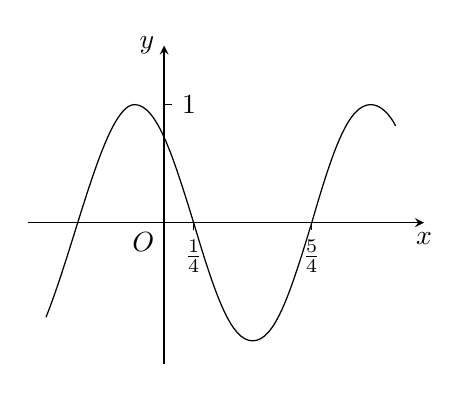
\begin{tikzpicture}[>=stealth,line width=.45pt,x=1.5cm,y=1.5cm]
  \draw[->] (-1.15,0) -- (2.2,0) node[below] {$x$};
  \draw[->] (0,-1.2) -- (0,1.5) node[left] {$y$};
  \node[below left] at (0,0) {$O$};
  \draw (0,1) -- (.07,1) node[right] {$1$};
  \draw (.25,0) -- (.25,-.06) node[below] {$\frac14$};
  \draw (1.25,0) -- (1.25,-.06) node[below] {$\frac54$};
  \draw (-1,-.8) .. controls (-.74,-.15) and (-.50,1) .. (-.25,1)
    .. controls (-.06,1) and (.08,.55) .. (.25,0)
    .. controls (.44,-.64) and (.57,-1) .. (.75,-1)
    .. controls (.94,-1) and (1.07,-.59) .. (1.25,0)
    .. controls (1.43,.62) and (1.56,1) .. (1.75,1)
    .. controls (1.83,1) and (1.91,.92) .. (1.96,.82);
\end{tikzpicture}
\end{center}
\nopagebreak[4]
(A) $\left(k\pi-\dfrac14,k\pi+\dfrac34\right),\ k\in\mathbb Z$　 (B) $\left(2k\pi-\dfrac14,2k\pi+\dfrac34\right),\ k\in\mathbb Z$

(C) $\left(k-\dfrac14,k+\dfrac34\right),\ k\in\mathbb Z$　 (D) $\left(2k-\dfrac14,2k+\dfrac34\right),\ k\in\mathbb Z$

\Needspace{0.4\textheight}
\end{question}
\begin{question}
\gkti{9}执行如图的程序框图，如果输入的 $t=0.01$，则输出的 $n=$（　）
\nopagebreak[4]
\begin{center}% source-figure:q09-flowchart, fixed science PDF p.1 / printed 961.
% Uses only basic TikZ paths and nodes; scaling/spacing are presentational.
\begin{tikzpicture}[>=stealth, every node/.style={font=\small}]
  \draw[rounded corners=5pt] (-0.52,0.05) rectangle (0.52,0.55);
  \node at (0,0.30) {开始};
  \draw[->] (0,0.05) -- (0,-0.45);
  \draw (-0.62,-0.45) -- (0.82,-0.45) -- (0.62,-0.95) -- (-0.82,-0.95) -- cycle;
  \node at (0,-0.70) {输入 $t$};
  \draw[->] (0,-0.95) -- (0,-1.45);
  \draw (-1.70,-1.45) rectangle (1.70,-2.00);
  \node at (0,-1.725) {$S=1,\ n=0,\ m=\frac12$};
  \draw[->] (0,-2.00) -- (0,-2.50);
  \draw (-0.92,-2.50) rectangle (0.92,-3.00);
  \node at (0,-2.75) {$S=S-m$};
  \draw[->] (0,-3.00) -- (0,-3.48);
  \draw (-1.50,-3.48) rectangle (1.50,-4.03);
  \node at (0,-3.755) {$m=\frac m2,\ n=n+1$};
  \draw[->] (0,-4.03) -- (0,-4.53);
  \draw (-1.08,-4.85) -- (0,-4.53) -- (1.08,-4.85) -- (0,-5.17) -- cycle;
  \node at (0,-4.85) {$S>t$};
  \draw[->] (-1.08,-4.85) -- (-2.05,-4.85) -- (-2.05,-2.25) -- (0,-2.25) -- (0,-2.50);
  \node[left] at (-1.08,-4.72) {是};
  \draw[->] (0,-5.17) -- (0,-5.65);
  \node[right] at (0.06,-5.40) {否};
  \draw (-0.62,-5.65) -- (0.82,-5.65) -- (0.62,-6.15) -- (-0.82,-6.15) -- cycle;
  \node at (0,-5.90) {输出 $n$};
  \draw[->] (0,-6.15) -- (0,-6.62);
  \draw[rounded corners=5pt] (-0.52,-7.12) rectangle (0.52,-6.62);
  \node at (0,-6.87) {结束};
\end{tikzpicture}
\end{center}
\nopagebreak[4]
(A) $5$　 (B) $6$　 (C) $7$　 (D) $8$

\end{question}
\begin{question}
\gkti{10}$(x^2+x+y)^5$ 的展开式中，$x^5y^2$ 的系数为（　）

(A) $10$　 (B) $20$　 (C) $30$　 (D) $60$

\Needspace{0.4\textheight}
\end{question}
\begin{question}
\gkti{11}圆柱被一个平面截去一部分后与半球（半径为 $r$）组成一个几何体，该几何体三视图中的正视图和俯视图如图所示．若该几何体的表面积为 $16+20\pi$，则 $r=$（　）
\nopagebreak[4]
\begin{center}% source-figure:q11-front, fixed science PDF p.1 / printed 961.
\begin{tikzpicture}[>=stealth,line width=.45pt]
  \draw (0,0) circle (1);
  \draw (-1,0) -- (1,0);
  \draw[thin] (-1,0) -- (-1,1.45) (1,0) -- (1,1.45);
  \draw[<->] (-1,1.25) -- (1,1.25) node[midway,above] {$2r$};
  \draw[thin] (1,0) -- (1.4,0) (0,-1) -- (1.4,-1);
  \draw[<->] (1.23,0) -- (1.23,-1) node[midway,right] {$r$};
  \node[below] at (0,-1.12) {正视图};
\end{tikzpicture}
\end{center}
\nopagebreak[4]
\nopagebreak[4]
\begin{center}% source-figure:q11-top, fixed science PDF p.1 / printed 961.
\begin{tikzpicture}[>=stealth,line width=.45pt]
  \draw (-1,0) arc[start angle=180,end angle=0,radius=1];
  \draw (-1,0) -- (1,0) -- (1,-2) -- (-1,-2) -- cycle;
  \draw[thin] (0,1) -- (-1.3,1) (-1,0) -- (-1.3,0);
  \draw[<->] (-1.2,0) -- (-1.2,1) node[midway,left] {$r$};
  \draw[thin] (1,0) -- (1.4,0) (1,-2) -- (1.4,-2);
  \draw[<->] (1.23,0) -- (1.23,-2) node[midway,right] {$2r$};
  \node[below] at (0,-2.12) {俯视图};
\end{tikzpicture}
\end{center}
\nopagebreak[4]
(A) $1$　 (B) $2$　 (C) $4$　 (D) $8$

\end{question}
\begin{question}
\gkti{12}设函数 $f(x)=e^x(2x-1)-ax+a$，其中 $a<1$，若存在唯一的整数 $x_0$ 使得 $f(x_0)<0$，则 $a$ 的取值范围是（　）

(A) $\left[-\dfrac{3}{2e},1\right)$　 (B) $\left[-\dfrac{3}{2e},\dfrac34\right)$　 (C) $\left[\dfrac{3}{2e},\dfrac34\right)$　 (D) $\left[\dfrac{3}{2e},1\right)$

\end{question}
\gkpart{二、填空题}

\begin{question}
\gkti{13}若函数 $f(x)=x\ln\!\left(x+\sqrt{a+x^2}\right)$ 为偶函数，则 $a=\underline{\qquad}$．

\end{question}
\begin{question}
\gkti{14}一个圆经过椭圆 $\dfrac{x^2}{16}+\dfrac{y^2}{4}=1$ 的三个顶点，且圆心在 $x$ 轴的正半轴上，则该圆的标准方程为 $\underline{\qquad}$．

\end{question}
\begin{question}
\gkti{15}若 $x,y$ 满足约束条件 $\begin{cases}x-1\geqslant0,\\x-y\leqslant0,\\x+y-4\leqslant0,\end{cases}$ 则 $\dfrac yx$ 的最大值为 $\underline{\qquad}$．

\end{question}
\begin{question}
\gkti{16}在平面四边形 $ABCD$ 中，$\angle A=\angle B=\angle C=75^\circ$，$BC=2$，则 $AB$ 的取值范围是 $\underline{\qquad}$．

\end{question}
\gkpart{三、解答题}

\begin{question}
\gkti{17}$S_n$ 为数列 $\{a_n\}$ 的前 $n$ 项和，已知 $a_n>0$，$a_n^2+2a_n=4S_n+3$．

(1) 求 $\{a_n\}$ 的通项公式；

(2) 设 $b_n=\dfrac1{a_na_{n+1}}$，求数列 $\{b_n\}$ 的前 $n$ 项和．

\Needspace{0.4\textheight}
\end{question}
\begin{question}
\gkti{18}如图，四边形 $ABCD$ 为菱形，$\angle ABC=120^\circ$，$E,F$ 是平面 $ABCD$ 同一侧的两点，$BE\perp$ 平面 $ABCD$，$DF\perp$ 平面 $ABCD$，$BE=2DF$，$AE\perp EC$．
\nopagebreak[4]
\begin{center}% source-figure:q18-solid, fixed science PDF p.1 / printed 961.
% Layout projection only; hidden AF changes style at its visible EC crossing.
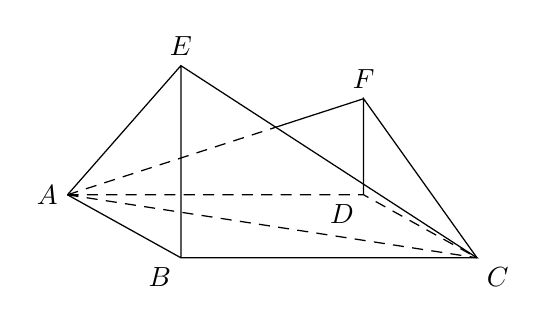
\begin{tikzpicture}[line width=.45pt,scale=.8]
  \coordinate (A) at (0,1);
  \coordinate (B) at (1.8,0);
  \coordinate (C) at (6.5,0);
  \coordinate (D) at (4.7,1);
  \coordinate (E) at (1.8,3.05);
  \coordinate (F) at (4.7,2.525);
  \coordinate (J) at (3.307,2.073);
  \draw (A) -- (B) -- (C) -- (E) -- (A) (E) -- (B);
  \draw (D) -- (F) -- (C) (J) -- (F);
  \draw[dash pattern=on 4pt off 3pt] (A) -- (J) (A) -- (D) -- (C) (A) -- (C);
  \node[left] at (A) {$A$};
  \node[below left] at (B) {$B$};
  \node[below right] at (C) {$C$};
  \node[below left] at (D) {$D$};
  \node[above] at (E) {$E$};
  \node[above] at (F) {$F$};
\end{tikzpicture}
\end{center}
\nopagebreak[4]
(1) 证明：平面 $AEC\perp$ 平面 $AFC$；

(2) 求直线 $AE$ 与直线 $CF$ 所成角的余弦值．

\Needspace{0.4\textheight}
\end{question}
\begin{question}
\gkti{19}某公司为确定下一年度投入某产品的宣传费，需了解年宣传费 $x$（单位：千元）对年销售量 $y$（单位：t）和年利润 $z$（单位：千元）的影响．对近 $8$ 年的年宣传费 $x_i$ 和年销售量 $y_i$（$i=1,2,\cdots,8$）数据作了初步处理，得到下面的散点图及一些统计量的值．
\nopagebreak[4]
\begin{center}% source-figure:q19-scatter, fixed science PDF p.2 / printed 962.
% Eight unlabelled squares are approximate visual placements, not raw data.
\begin{tikzpicture}[>=stealth,line width=.4pt,x=.23cm,y=.023cm,
  every node/.style={font=\small}]
  \draw[->] (34,480) -- (62,480);
  \draw[->] (34,480) -- (34,640);
  \foreach \x in {34,36,...,56} {
    \draw (\x,480) -- (\x,484);
    \node[below] at (\x,480) {\x};
  }
  \foreach \y in {480,500,...,620} {
    \draw (34,\y) -- (34.4,\y);
    \node[left] at (34,\y) {\y};
  }
  \node[above right] at (34,635) {年销售量/t};
  \node[above] at (62,480) {年宣传费/千元};
  \foreach \x/\y in {38/502,40/534,44/564,46/576,48/590,50/596,52/600,56/604} {
    \fill (\x,\y) ++(-1pt,-1pt) rectangle ++(2pt,2pt);
  }
\end{tikzpicture}
\end{center}
\nopagebreak[4]
\begin{center}
\begin{tabular}{rrrrr}
\toprule
$\overline x$ & $\overline y$ & $\overline w$ & $\sum_{i=1}^{8}(x_i-\overline x)^2$ & $\sum_{i=1}^{8}(w_i-\overline w)^2$ \\
\midrule
$46.6$ & $563$ & $6.8$ & $289.8$ & $1.6$ \\
\bottomrule
\end{tabular}
\end{center}

\begin{center}
\begin{tabular}{rr}
\toprule
$\sum_{i=1}^{8}(x_i-\overline x)(y_i-\overline y)$ & $\sum_{i=1}^{8}(w_i-\overline w)(y_i-\overline y)$ \\
\midrule
$1.469$ & $108.8$ \\
\bottomrule
\end{tabular}
\end{center}

表中 $w_i=\sqrt{x_i}$，$\overline w=\dfrac18\sum_{i=1}^{8}w_i$．

(1) 根据散点图判断，$y=a+bx$ 与 $y=c+d\sqrt x$ 哪一个适宜作为年销售量 $y$ 关于年宣传费 $x$ 的回归方程类型？（给出判断即可，不必说明理由）

(2) 根据 (1) 的判断结果及表中数据，建立 $y$ 关于 $x$ 的回归方程；

(3) 已知这种产品的年利润 $z$ 与 $x,y$ 的关系为 $z=0.2y-x$．根据 (2) 的结果回答下列问题：

① 年宣传费 $x=49$ 时，年销售量及年利润的预报值是多少？

② 年宣传费 $x$ 为何值时，年利润的预报值最大？

附：对于一组数据 $(u_1,v_1),(u_2,v_2),\cdots,(u_n,v_n)$，其回归直线 $v=\alpha+\beta u$ 的斜率和截距的最小二乘估计分别为 $\widehat\beta=\dfrac{\sum_{i=1}^{n}(u_i-\overline u)(v_i-\overline v)}{\sum_{i=1}^{n}(u_i-\overline u)^2}$，$\widehat\alpha=\overline v-\widehat\beta\,\overline u$．

\end{question}
\begin{question}
\gkti{20}在直角坐标系 $xOy$ 中，曲线 $C:y=\dfrac{x^2}{4}$ 与直线 $l:y=kx+a$（$a>0$）交于 $M,N$ 两点．

(1) 当 $k=0$ 时，分别求 $C$ 在点 $M$ 和 $N$ 处的切线方程；

(2) $y$ 轴上是否存在点 $P$，使得当 $k$ 变动时，总有 $\angle OPM=\angle OPN$？说明理由．

\end{question}
\begin{question}
\gkti{21}已知函数 $f(x)=x^3+ax+\dfrac14$，$g(x)=-\ln x$．

(1) 当 $a$ 为何值时，$x$ 轴为曲线 $y=f(x)$ 的切线；

(2) 用 $\min\{m,n\}$ 表示 $m,n$ 中的最小值，设函数 $h(x)=\min\{f(x),g(x)\}$（$x>0$），讨论 $h(x)$ 零点的个数．

\Needspace{0.4\textheight}
\end{question}
\begin{question}
\gkti{22}如图，$AB$ 是 $\odot O$ 的直径，$AC$ 是 $\odot O$ 的切线，$BC$ 交 $\odot O$ 于点 $E$．
\nopagebreak[4]
\begin{center}% source-figure:q22-circle, fixed science PDF p.2 / printed 962.
% Layout-only circle/secant construction; DE is visible in the source.
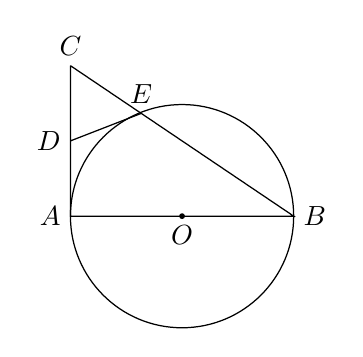
\begin{tikzpicture}[line width=.45pt,scale=1.05]
  \coordinate (A) at (-1.35,0);
  \coordinate (B) at (1.35,0);
  \coordinate (C) at (-1.35,1.82);
  \coordinate (D) at (-1.35,.91);
  \coordinate (E) at (-.4935,1.2426);
  \draw (0,0) circle (1.35);
  \draw (C) -- (A) -- (B) -- (C) (D) -- (E);
  \fill (0,0) circle (1pt);
  \node[left] at (A) {$A$};
  \node[right] at (B) {$B$};
  \node[above] at (C) {$C$};
  \node[left] at (D) {$D$};
  \node[above] at (E) {$E$};
  \node[below] at (0,0) {$O$};
\end{tikzpicture}
\end{center}
\nopagebreak[4]
(1) 若 $D$ 为 $AC$ 的中点，证明：$DE$ 是 $\odot O$ 的切线；

(2) 若 $OA=\sqrt3 CE$，求 $\angle ACB$ 的大小．

\end{question}
\begin{question}
\gkti{23}在直角坐标系 $xOy$ 中，直线 $C_1:x=-2$，圆 $C_2:(x-1)^2+(y-2)^2=1$，以坐标原点为极点，$x$ 轴的正半轴为极轴建立极坐标系．

(1) 求 $C_1,C_2$ 的极坐标方程；

(2) 若直线 $C_3$ 的极坐标方程为 $\theta=\dfrac\pi4$（$\rho\in\mathbb R$），设 $C_2$ 与 $C_3$ 的交点为 $M,N$，求 $\triangle C_2MN$ 的面积．

\end{question}
\begin{question}
\gkti{24}已知函数 $f(x)=|x+1|-2|x-a|$，$a>0$．

(1) 当 $a=1$ 时，求不等式 $f(x)>1$ 的解集；

(2) 若 $f(x)$ 的图象与 $x$ 轴围成的三角形面积大于 $6$，求 $a$ 的取值范围．

\end{question}